\documentclass[twocolumn]{article}
\usepackage[utf8]{inputenc}
\usepackage{graphicx}
\graphicspath{{figures/}}
\usepackage{natbib}
\usepackage{times}
\usepackage{url}
\usepackage[margin=0.75in]{geometry}
\usepackage{caption}
\usepackage{float}
\usepackage{booktabs}
\usepackage{amsmath}
\usepackage{xcolor}
\usepackage{tikz}
\usetikzlibrary{shapes.geometric, arrows.meta, positioning}

% Several figures are generated by the accompanying scripts (visualizer.py,
% train.py, evaluate.py, gradcam.py). \genfigure falls back to a labeled
% placeholder box if a figure has not been generated yet, so the paper always
% compiles, and picks up the real image automatically once it exists.
\newcommand{\genfigure}[3]{%
  \IfFileExists{figures/#1}{%
    \includegraphics[width=#2]{#1}%
  }{%
    \fbox{\parbox[c][3.2cm]{#2}{\centering\itshape #3}}%
  }%
}

\title{\textbf{Brain Tumor Classification with Pretrained CNNs in PyTorch}}
\author{Jaiveer Bassi \\
\texttt{jaiveerbassi@yahoo.com}}
\date{}

\begin{document}

\maketitle

\begin{abstract}
Brain tumors need to be diagnosed quickly and correctly, and manual review of MRI scans by radiologists, while accurate, is slow and can vary from one reader to another. Convolutional neural networks (CNNs) offer a way to automate part of this process and support, rather than replace, clinical judgment. This paper does two things. First, it presents a complete and reproducible transfer learning pipeline that sorts brain MRI scans into four categories using a fine-tuned ResNet-18: on a held-out test set of 1,311 images it reaches 99.16\% accuracy, and across five random seeds 99.16\% with a standard deviation of 0.14 points. Second, and more importantly, it audits the widely used public dataset the pipeline is trained on, and reports two findings that users of this benchmark should know. The dataset's train and test splits overlap heavily: 216 test images (16.5\%) are pixel-identical to a training image and 103 are byte-identical files, with a further 207 duplicates inside the training split. Separately, we could not verify the commonly repeated claim that this collection derives from the figshare brain tumor dataset; matching all 5,023 tumor images against all 3,064 figshare slices, under a rendering-invariant test whose positive control scores 1.0000, produced no correspondence above 0.87. The natural inference from the first finding turns out to be wrong, and this is the result we most want to record: removing the duplicates does not reduce measured accuracy. Retraining on a deduplicated split gives 99.23\% $\pm$ 0.29 against 99.16\% $\pm$ 0.14 on the original split, a difference of 0.07 points in the wrong direction for the leakage hypothesis and far from significant ($p = 0.65$). The near-ceiling accuracy on this benchmark is therefore not an artifact of duplicate contamination, though the contamination is real, undocumented, and does appear to suppress the apparent run-to-run variance. We also report per-class metrics, an ablation isolating a 15.6-point effect of full fine-tuning, temperature-scaled calibration, and Grad-CAM interpretability. All code, figures, audit tooling, and hyperparameters are released so every number here can be reproduced on a single consumer GPU.
\end{abstract}

\section{Introduction}
A brain tumor is an abnormal growth of cells inside the skull, and depending on type and location, it can be life-threatening. Tumors are classified as primary, meaning they originate in the brain, or secondary, meaning they spread from cancer elsewhere in the body. Among primary tumors, gliomas and meningiomas are the most common, with gliomas generally being more aggressive. Because symptoms depend heavily on tumor size and location, early and accurate detection matters a great deal. Diagnosis has traditionally relied on radiologists reading MRI scans by hand, a process that takes time and is subject to disagreement between readers. Given how much a delayed or missed diagnosis can affect a patient's outcome, there is real value in tools that can support this process.

Deep learning, and CNNs in particular, has changed how image analysis is done by learning hierarchical features directly from pixels instead of relying on hand-crafted rules. This has made it possible to segment and classify medical images without manually engineering features for every task. When labeled data is limited, which is common in medical imaging, transfer learning helps close the gap: a CNN pretrained on a large natural-image dataset like ImageNet is fine-tuned on the smaller medical dataset instead of being trained from nothing. \citet{tajbakhsh2016convolutional} showed that fine-tuned pretrained models frequently outperform models trained from scratch on medical imaging tasks. CNNs have since been applied widely to both segmentation and classification of brain MRI. \citet{havaei2017brain}, for example, combined local and global image context in a single CNN to achieve strong glioblastoma segmentation results. On the classification side, several recent studies report high accuracy with transfer learning: \citet{disci2023fine} fine-tuned architectures such as Xception, MobileNetV2, InceptionV3, ResNet50, VGG16, and DenseNet121 on the same four-class dataset used here and reported strong classification accuracy, while \citet{vimala2023efficientnet} used a hybrid deep learning approach to reach high test accuracy distinguishing glioma, meningioma, and pituitary tumors.

The contribution of this paper is not a new architecture. It is a clean, fully documented baseline, plus an audit of the benchmark that baseline is measured on. Specifically:

\begin{itemize}
\itemsep0.2em
\item We describe the entire pipeline end to end, from folder layout and preprocessing through training, evaluation, and interpretability, with every hyperparameter stated (Sections~\ref{sec:method} and~\ref{sec:setup}).
\item We document substantial duplicate contamination between the dataset's train and test splits, at three levels of strictness, with visual evidence (Section~\ref{sec:contamination}).
\item We investigate the dataset's provenance and report that the commonly repeated attribution to the figshare collection of \citet{cheng2015enhanced} could not be verified by content matching (Section~\ref{sec:provenance}).
\item We test the obvious consequence of the contamination and find it does not hold: retraining on a deduplicated split leaves accuracy statistically unchanged (Section~\ref{sec:dedup}). We think this negative result matters more than the contamination itself, because it is the conclusion a reader would otherwise assume without checking.
\item We report complete results rather than a headline accuracy: per-class precision, recall, and F1, the raw confusion matrix, per-class ROC-AUC, and an analysis of every test-set error (Section~\ref{sec:results}).
\item We measure run-to-run noise with a five-seed sweep on both splits, and isolate the effect of augmentation and fine-tuning strategy with an ablation (Section~\ref{sec:variance}).
\item We test whether the model's confidence can be trusted using temperature scaling, and report a concrete, honest result rather than assuming calibration is fine (Section~\ref{sec:calibration}).
\item We include Grad-CAM interpretability and use it to check that the model attends to anatomically plausible regions (Section~\ref{sec:interpretability}).
\end{itemize}

A note on how to read the accuracy figures in this paper. Because the benchmark is saturated and, as we show, contaminated, we do not think 99\% on it is evidence that the problem is solved. The numbers are reported so that others can reproduce them and so that the deduplication comparison has a baseline, not as a claim of clinical readiness.

\section{Related Work}
CNNs have performed well across a range of medical imaging tasks, including tumor segmentation and detection. \citet{havaei2017brain} introduced a fully automatic brain tumor segmentation network that improved both speed and accuracy over earlier methods by combining local and more global contextual features. \citet{pereira2016brain} took a related approach, building a deep CNN for glioma segmentation using small convolutional kernels stacked in depth. These segmentation studies motivate our use of CNNs for classification, since the same hierarchical features that trace tumor boundaries can plausibly distinguish between tumor types.

Transfer learning is a natural fit for classification problems with limited labeled data. \citet{tajbakhsh2016convolutional} studied medical image analysis tasks spanning radiology and cardiology and found that CNNs pretrained on ImageNet and then fine-tuned generally outperform networks trained from scratch, and that fine-tuned networks are also more robust when training data is scarce. MRI scans look nothing like ImageNet's natural photographs, but this line of work is exactly why we still start from an ImageNet-pretrained ResNet-18: fine-tuning lets the network adapt its low-level filters to MRI texture while keeping the general-purpose pattern detectors learned from a much larger dataset.

A large share of this literature builds on the T1-weighted contrast-enhanced brain tumor dataset released by \citet{cheng2015enhanced} on Figshare, which covers the same three tumor types (glioma, meningioma, pituitary) used here and has become a de facto benchmark; several of the public four-class collections used in more recent work, including datasets used by studies discussed below, trace part of their images back to it. \citet{swati2019brain} were among the first to apply transfer learning to this dataset directly, using a block-wise fine-tuning strategy on a pretrained VGG19 rather than fine-tuning the whole network at once, which let them study how much of a pretrained CNN actually needs to change for a new imaging domain. \citet{deepak2019brain} took a feature-extraction approach instead, using a pretrained GoogLeNet purely to produce features and training a separate classifier on top, and reported a mean classification accuracy of 98\% across glioma, meningioma, and pituitary tumors. \citet{khan2020brain} trained a CNN classifier on a smaller, independently annotated brain MRI collection, which is a useful reminder that results on the large aggregated datasets used elsewhere in this section do not automatically transfer to differently sourced data.

Several more recent studies broaden the comparison to more backbones or add a second technique on top of transfer learning. \citet{disci2023fine} benchmarked six pretrained architectures, including Xception, ResNet50, and DenseNet121, on the same public four-class brain MRI dataset used in this paper and reported strong classification accuracy through transfer learning and fine-tuning. \citet{vimala2023efficientnet} applied a hybrid deep learning approach combining EfficientNet-based transfer learning with additional classifiers on the Figshare brain tumor dataset and reported high accuracy across glioma, meningioma, and pituitary tumor classes. \citet{srinivas2022deep} compared VGG-16, ResNet-50, and Inception-v3 directly against each other under the same transfer learning setup and found meaningful accuracy differences between backbones on the same data, which is a useful caution against assuming any one pretrained network is the right default choice. \citet{krishnapriya2023pretrained} ran a similar head-to-head comparison across a wider set of pretrained models. \citet{anaya2023optimizing} went further and compared standard transfer learning against data augmentation and a cross-transformer architecture on the same classification and detection tasks, which starts to probe whether the gains in this literature come from the backbone, the augmentation, or the training recipe. \citet{dutta2022multi} is a smaller-scale study in the same vein, applying transfer learning-based deep networks to the multi-class version of the problem. Other work looks at combining models rather than picking one: \citet{chen2024fusion} fused deep features from multiple pretrained CNNs to improve the robustness of multi-type brain tumor classification, reporting accuracy above 95\% on their evaluation set; \citet{sankar2024efficient} built an ensemble of deep learning models specifically for tumor \emph{grade} classification, a related but distinct problem from the type classification addressed here; \citet{gasmi2024enhanced} combined several deep models with a weight-selection technique to merge their predictions; and \citet{alkharaan2026brain} paired an EfficientNet classifier with a U-Net++ segmentation branch so that classification and tumor localization are produced together rather than as separate steps.

Taken together, these results suggest that pretrained CNNs, given careful fine-tuning and reasonable data augmentation, can classify brain tumors with high accuracy across a wide range of backbones and training recipes. What is often missing from these reports is the detail needed to reproduce them exactly: full hyperparameters, a fixed held-out test set that is never touched during model selection, a complete confusion matrix rather than a single accuracy figure, and code that is actually released. That gap is what this paper tries to fill.

\section{Dataset and Audit}
\label{sec:dataset}
We use the brain MRI dataset released by \citet{ghaffar2020dataset} on Mendeley Data in 2024, which contains 7,023 T1-weighted, contrast-enhanced MRI images spanning four classes: glioma, meningioma, pituitary tumor, and no tumor. The images are JPEG-formatted axial and coronal slices, gathered from multiple sources and pre-split by the dataset authors into training and testing folders. That split matters for evaluation: our pipeline treats the training folder as the only source of trainable data and keeps the testing folder completely untouched until final evaluation, so no test image influences either the weights or the choice of checkpoint.

Table~\ref{tab:dataset} gives the exact composition of both splits as counted directly from disk. The classes are reasonably balanced, with \texttt{notumor} the largest at 1,595 training images and \texttt{glioma} the smallest at 1,321. Figure~\ref{fig:samples} shows example scans from each class, and Figure~\ref{fig:class_dist} plots the same counts visually. Both figures are generated by \texttt{visualizer.py} from whatever copy of the data is on disk rather than hardcoded, so they always describe the data actually being trained on.

\begin{table}[H]
\centering
\caption{Dataset composition, counted from disk. The training split is further divided 80/20 into 4,569 training and 1,143 validation images.}
\label{tab:dataset}
\begin{tabular}{lrrr}
\toprule
Class & Training & Testing & Total \\
\midrule
glioma      & 1,321 & 300 & 1,621 \\
meningioma  & 1,339 & 306 & 1,645 \\
notumor     & 1,595 & 405 & 2,000 \\
pituitary   & 1,457 & 300 & 1,757 \\
\midrule
Total       & 5,712 & 1,311 & 7,023 \\
\bottomrule
\end{tabular}
\end{table}

\begin{figure}[H]
    \centering
    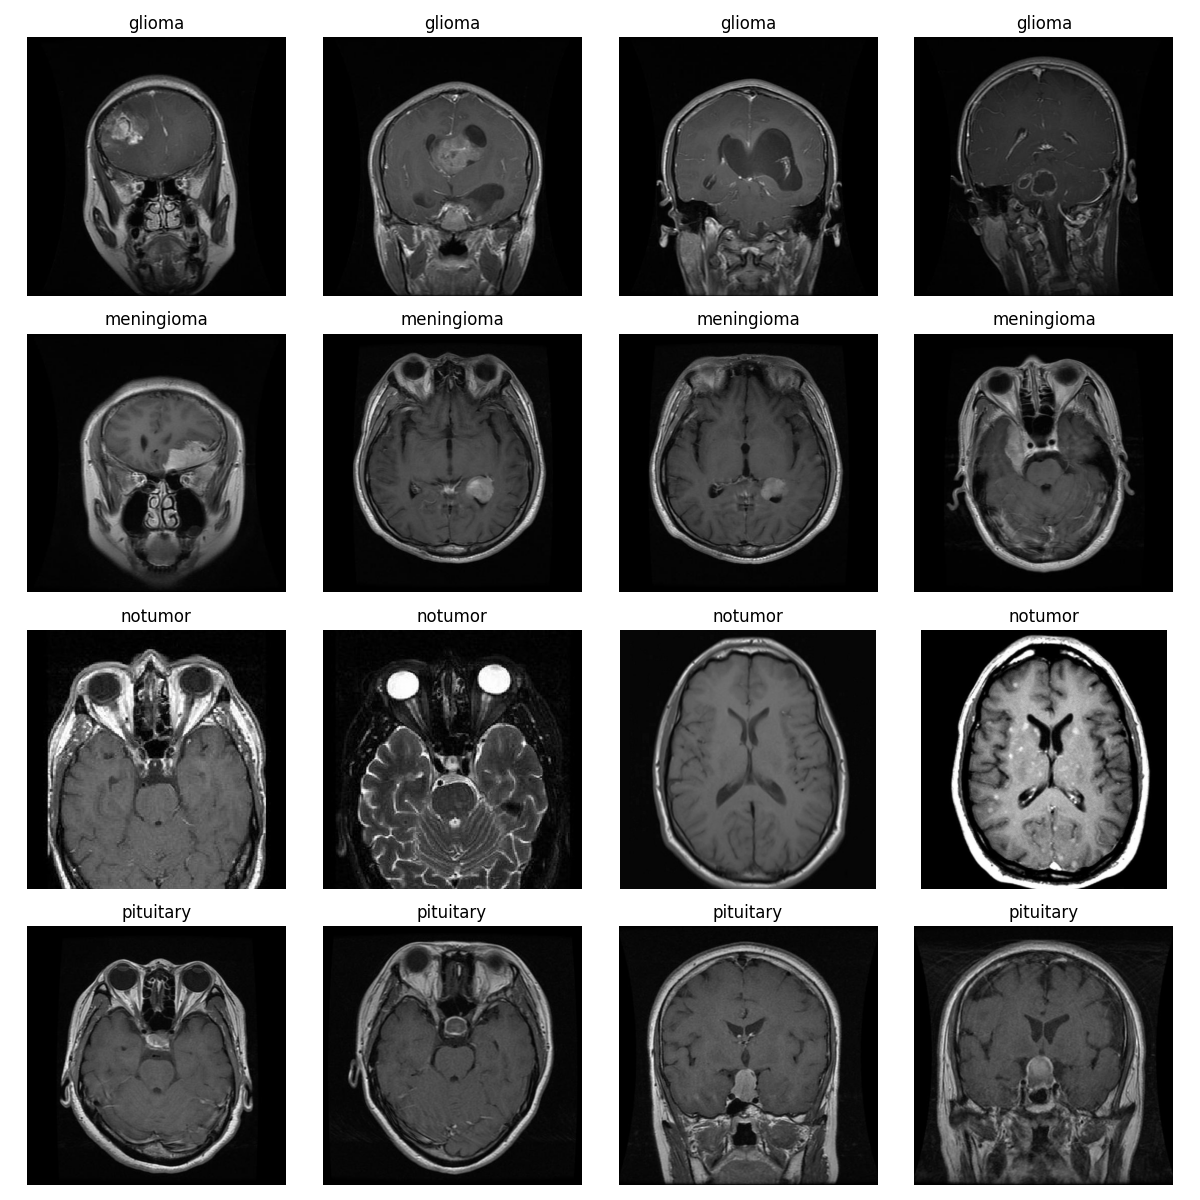
\includegraphics[width=0.9\linewidth]{Figure_1.png}
    \caption{Sample MRI scans from each of the four classes.}
    \label{fig:samples}
\end{figure}

\begin{figure}[H]
    \centering
    \genfigure{class_distribution.png}{0.9\linewidth}{Run \texttt{visualizer.py --data\_dir <path> --save} to generate this figure.}
    \caption{Number of images per class in the training and testing splits, generated by \texttt{visualizer.py}.}
    \label{fig:class_dist}
\end{figure}

To match ImageNet-pretrained models such as ResNet-18, every image is resized to $224 \times 224$ and grayscale scans are copied across three channels to look like RGB input. Pixel values are then normalized using ImageNet's mean and standard deviation so the pretrained convolutional filters and batch-normalization statistics behave as intended. This dataset is used widely for benchmarking brain tumor classification \citep{disci2023fine, vimala2023efficientnet}, and its open access and balanced classes make it a practical choice for reproducible research.

That popularity is why the rest of this section is worth the space. Before reporting any accuracy on this benchmark, we audited it, and found two things that anyone using it should know: its train and test splits overlap substantially, and its provenance does not appear to be what it is commonly said to be.

\subsection{Provenance}
\label{sec:provenance}
Aggregated brain MRI collections of this shape are widely described as combinations of three public sources: the T1-weighted contrast-enhanced dataset of \citet{cheng2015enhanced}, the SARTAJ collection, and the Br35H set of normal scans. If the tumor classes here derive from \citet{cheng2015enhanced}, that would matter a great deal for evaluation, because that release stores a patient identifier with each of its 3,064 slices and contains multiple slices per patient. A split made by shuffling slices rather than by patient would then place the same patient on both sides of the train/test boundary, and the test set would no longer measure generalization to unseen patients.

We tried to establish this directly. We downloaded all 3,064 figshare slices (233 patients) and rendered each one to 8-bit using exactly the conversion the dataset's own README documents, then matched all 5,023 tumor-class images in our copy against all 3,064 slices. We used three independent measures: cosine similarity of ImageNet-pretrained ResNet-18 features, correlation after per-image histogram equalization (which is invariant to any monotonic intensity remapping, so a different windowing choice cannot defeat it), and intersection-over-union of binarized brain masks (which survives intensity changes and moderate cropping). As a positive control, we ran the same measures on a pair of images known to be identical, taken from the contamination analysis in Section~\ref{sec:contamination}.

The positive control scores 1.0000 on both equalized correlation and mask IoU, so the measures do reach unity for a true match. Against figshare, nothing comes close. The best equalized correlation over all 5,023 by 3,064 comparisons is 0.872, with nothing above 0.90; the best embedding cosine is 0.963, with nothing above 0.98; the best mask IoU is 0.938. For scale, randomly chosen pairs of unrelated images from within our own dataset reach a median best-match correlation of 0.838. In other words, figshare slices resemble these tumor images no more than two arbitrary brain MRIs resemble each other. The class counts point the same way: figshare contains 708 meningioma slices, while this dataset contains 1,645.

We therefore report a negative result. We cannot confirm that the tumor images in this dataset come from \citet{cheng2015enhanced}, and the evidence weighs against it. This has a practical consequence: no patient identifiers are recoverable for these images from that source, so a patient-disjoint split cannot be constructed for this benchmark, and no study using it can claim patient-level separation. We restrict this claim to the figshare component, which is the only one we tested directly; we did not attempt to verify or rule out the SARTAJ and Br35H attributions. We also note the caveat that an undocumented and aggressive preprocessing step, such as skull-stripping or resampling, could in principle defeat even mask IoU. We consider that unlikely given the visual similarity in framing and field of view, but we cannot exclude it.

\subsection{Duplicate Contamination}
\label{sec:contamination}
The second finding needs no thresholds to state. We hashed every image in both splits, first by raw file bytes and then by decoded pixel content at a fixed resolution, so that an image re-encoded at a different JPEG quality still collides with its original. Table~\ref{tab:contamination} reports the result.

\begin{table}[H]
\centering
\caption{Duplicate contamination in the released split. Percentages are of the 1,311-image test set.}
\label{tab:contamination}
\small
\begin{tabular}{lrr}
\toprule
Category & Count & \% of test \\
\midrule
Byte-identical test/train files & 103 & 7.9\% \\
Pixel-identical test/train images & 216 & 16.5\% \\
Duplicates within training split & 207 & \\
Duplicates within test split & 30 & 2.3\% \\
\bottomrule
\end{tabular}
\end{table}

216 of the 1,311 test images, 16.5\% of the test set, are pixel-for-pixel the same image as something the model trains on, and 103 of those are identical at the level of the file itself. We verified a sample byte for byte. Figure~\ref{fig:leakage} shows examples: these are not similar patients or adjacent slices, they are the same scan appearing twice.

\begin{figure}[H]
    \centering
    \genfigure{leakage_examples.png}{0.98\linewidth}{Run \texttt{audit\_leakage.py} to generate this figure.}
    \caption{Test images (left of each pair) beside their nearest training image. Every pair shown is pixel-identical. Generated by \texttt{audit\_leakage.py}.}
    \label{fig:leakage}
\end{figure}

The contamination is very unevenly distributed across classes, which turns out to matter for interpreting the results later. Table~\ref{tab:contamclass} breaks it down. The \texttt{notumor} class is the worst affected in absolute terms, and \texttt{glioma} is essentially untouched: not one glioma test image duplicates a training image.

\begin{table}[H]
\centering
\caption{Pixel-identical duplicates by class. Test column counts test images duplicating some training image.}
\label{tab:contamclass}
\small
\begin{tabular}{lrrr}
\toprule
Class & Test dupes & \% of class & Within train \\
\midrule
glioma      & 0   & 0.0\%  & 0   \\
meningioma  & 106 & 34.6\% & 6   \\
notumor     & 105 & 25.9\% & 189 \\
pituitary   & 5   & 1.7\%  & 12  \\
\bottomrule
\end{tabular}
\end{table}

Relaxing to near-duplicates rather than exact ones, 200 further test images sit at cosine similarity 0.99 or above to a training image without being pixel-identical, 197 of them in \texttt{notumor}. We treat that number with more caution than the exact counts, because brain MRI slices are generically similar to one another: in our data the nearest different-class training image already sits at roughly 0.90 cosine, so the metric is not sharply discriminative and the threshold is a judgment call. The exact-duplicate counts require no such judgment, and they are what we rely on.

The redundancy of the \texttt{notumor} class deserves a separate mention. It contributes 189 of the 207 within-train duplicates and 197 of the 200 near-duplicates, and relaxing the criterion to cosine 0.99 removes 75\% of its test images. Whatever its source, this class contains far less independent information than its raw count of 2,000 images suggests.

\section{Methodology}
\label{sec:method}
Figure~\ref{fig:pipeline} outlines the full pipeline. An input MRI scan is preprocessed to match the format ResNet-18 expects, passed through the pretrained backbone and a newly initialized four-class head, and converted to class probabilities. The resulting predictions feed both the quantitative evaluation and the Grad-CAM interpretability step described in Sections~\ref{sec:results} and~\ref{sec:interpretability}.

\begin{figure*}[t]
\centering
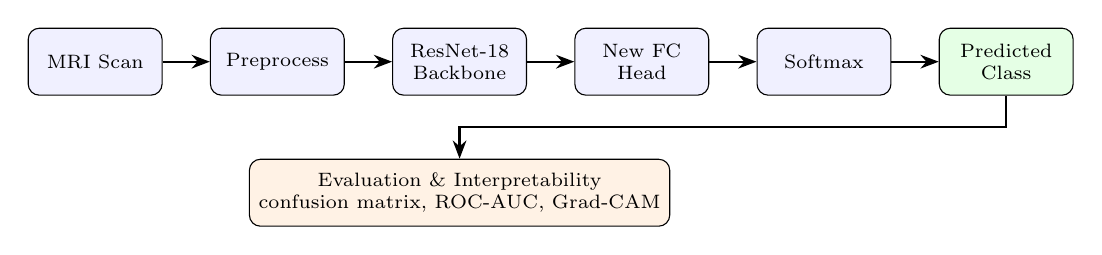
\begin{tikzpicture}[
  node distance=4mm and 6mm,
  box/.style={draw, rounded corners, minimum height=0.85cm, minimum width=1.7cm, align=center, font=\scriptsize, fill=blue!6},
  arr/.style={-Stealth, thick}
]
\node[box] (input) {MRI Scan};
\node[box, right=of input] (prep) {Preprocess};
\node[box, right=of prep] (backbone) {ResNet-18\\Backbone};
\node[box, right=of backbone] (head) {New FC\\Head};
\node[box, right=of head] (softmax) {Softmax};
\node[box, right=of softmax, fill=green!10] (pred) {Predicted\\Class};

\draw[arr] (input) -- (prep);
\draw[arr] (prep) -- (backbone);
\draw[arr] (backbone) -- (head);
\draw[arr] (head) -- (softmax);
\draw[arr] (softmax) -- (pred);

\node[box, below=8mm of backbone, fill=orange!10, minimum width=3.6cm] (evalbox) {Evaluation \& Interpretability\\confusion matrix, ROC-AUC, Grad-CAM};
\draw[arr] (pred.south) -- ++(0,-4mm) -| (evalbox.north);
\end{tikzpicture}
\caption{End-to-end pipeline. Preprocessing, the ResNet-18 backbone, and the new classification head are described in Sections~\ref{sec:preprocessing} and~\ref{sec:architecture}; evaluation and interpretability are described in Sections~\ref{sec:results} and~\ref{sec:interpretability}.}
\label{fig:pipeline}
\end{figure*}

Because pretrained CNNs offer a strong balance of representational power and computational cost, we build on ResNet-18 \citep{he2016deep} throughout, though the accompanying code also supports ResNet-34 and EfficientNet-B0 as drop-in alternatives.

\subsection{Data Preprocessing}
\label{sec:preprocessing}
Figure~\ref{fig:preprocessing} shows the preprocessing chain. All MRI images are resized to $224 \times 224$ pixels to match ResNet-18's expected input. Since the source images are grayscale, the single channel is duplicated three times to imitate an RGB image. Pixel values are then normalized using ImageNet's mean (0.485, 0.456, 0.406) and standard deviation (0.229, 0.224, 0.225). These steps keep the pretrained model's early filters and batch-normalization statistics operating in the input range they were trained on. When augmentation is enabled, a random horizontal flip, a rotation of up to 10 degrees, and brightness and contrast jitter of up to 10\% are applied before normalization. None of these transformations change the diagnostic label of the scan, which is what makes them safe to use here.

\begin{figure}[H]
\centering
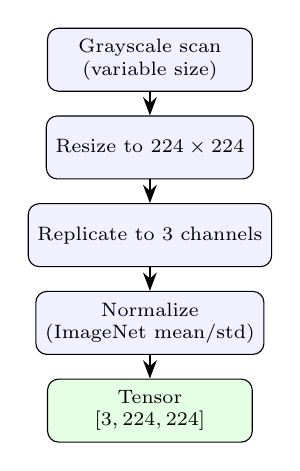
\begin{tikzpicture}[
  node distance=3mm,
  box/.style={draw, rounded corners, minimum height=0.8cm, minimum width=2.6cm, align=center, font=\scriptsize, fill=blue!6},
  arr/.style={-Stealth, thick}
]
\node[box] (raw) {Grayscale scan\\(variable size)};
\node[box, below=of raw] (resize) {Resize to $224\times224$};
\node[box, below=of resize] (chan) {Replicate to 3 channels};
\node[box, below=of chan] (norm) {Normalize\\(ImageNet mean/std)};
\node[box, below=of norm, fill=green!10] (tensor) {Tensor\\$[3, 224, 224]$};

\draw[arr] (raw) -- (resize);
\draw[arr] (resize) -- (chan);
\draw[arr] (chan) -- (norm);
\draw[arr] (norm) -- (tensor);
\end{tikzpicture}
\caption{Preprocessing steps applied to every scan before it reaches the network.}
\label{fig:preprocessing}
\end{figure}

\subsection{Model Architecture}
\label{sec:architecture}
We use ResNet-18 as implemented in \texttt{torchvision.models}, pretrained on ImageNet. Figure~\ref{fig:architecture} shows the layout: the convolutional stem and four residual stages carry over their pretrained weights, and the final fully connected layer, originally sized for 1,000 ImageNet classes, is replaced with a new linear layer with four outputs, one per tumor class. The entire network is fine-tuned rather than just the new head, since full fine-tuning has been shown to outperform freezing early layers on many medical imaging tasks \citep{tajbakhsh2016convolutional}. The code also supports freezing the backbone (\texttt{--freeze\_backbone}) for faster experimentation on smaller GPUs.

\begin{figure}[H]
\centering
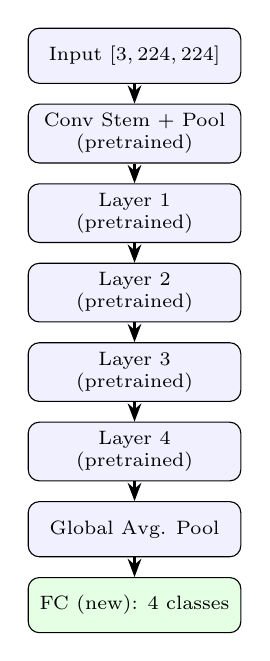
\begin{tikzpicture}[
  node distance=2.5mm,
  box/.style={draw, rounded corners, minimum height=0.7cm, minimum width=2.7cm, align=center, font=\scriptsize, fill=blue!6},
  arr/.style={-Stealth, thick}
]
\node[box] (in) {Input $[3,224,224]$};
\node[box, below=of in] (stem) {Conv Stem + Pool\\(pretrained)};
\node[box, below=of stem] (l1) {Layer 1\\(pretrained)};
\node[box, below=of l1] (l2) {Layer 2\\(pretrained)};
\node[box, below=of l2] (l3) {Layer 3\\(pretrained)};
\node[box, below=of l3] (l4) {Layer 4\\(pretrained)};
\node[box, below=of l4] (gap) {Global Avg. Pool};
\node[box, below=of gap, fill=green!10] (fc) {FC (new): 4 classes};

\draw[arr] (in) -- (stem);
\draw[arr] (stem) -- (l1);
\draw[arr] (l1) -- (l2);
\draw[arr] (l2) -- (l3);
\draw[arr] (l3) -- (l4);
\draw[arr] (l4) -- (gap);
\draw[arr] (gap) -- (fc);
\end{tikzpicture}
\caption{ResNet-18 with its final layer replaced. Blue blocks keep their ImageNet-pretrained weights and are fine-tuned; the green block is initialized from scratch. Layer 4 is also the target layer for Grad-CAM.}
\label{fig:architecture}
\end{figure}

\subsection{Training Procedure}
Training uses cross-entropy loss and the Adam optimizer. The official training folder is split with a stratified 80/20 partition so each class appears in the same proportion in both subsets, giving 4,569 training and 1,143 validation images. A \texttt{ReduceLROnPlateau} scheduler halves the learning rate when validation loss stops improving for two epochs, and training stops early if validation loss fails to improve for five consecutive epochs. The checkpoint is saved whenever validation loss reaches a new minimum, so the model that gets evaluated is the best one seen during training and not simply the last one. All random number generators are seeded, and the checkpoint stores the class names and backbone choice alongside the weights, so evaluation and inference never have to guess the class order.

\section{Experimental Setup}
\label{sec:setup}
Table~\ref{tab:hyper} lists every hyperparameter used to produce the results in this paper. Training ran on a single NVIDIA RTX 4070 with PyTorch 2.14 and CUDA 12.6, and each run completed in between roughly 8 and 20 minutes; the same script runs unchanged on CPU, just considerably slower. Evaluation metrics come from \texttt{scikit-learn}, and every figure and table in this paper is produced directly by the released scripts.

The main result (Table~\ref{tab:results} onward) uses seed 42. Section~\ref{sec:variance} reports five-seed and ablation runs produced by \texttt{train.py} with different \texttt{--seed}, \texttt{--augment}, and \texttt{--freeze\_backbone} settings, orchestrated by \texttt{run\_seed\_sweep.py}. Section~\ref{sec:calibration} uses \texttt{calibrate.py} to fit and evaluate temperature scaling. The audit in Section~\ref{sec:contamination} is produced by \texttt{audit\_leakage.py}, the provenance analysis in Section~\ref{sec:provenance} by \texttt{match\_figshare.py}, and the deduplicated split in Section~\ref{sec:dedup} by \texttt{build\_clean\_split.py}. Every per-run metric behind every table is written to JSON by those scripts and included in the repository, so the aggregate numbers can be checked without rerunning anything.

\begin{table}[H]
\centering
\caption{Hyperparameters used for the reported run.}
\label{tab:hyper}
\begin{tabular}{ll}
\toprule
Setting & Value \\
\midrule
Backbone & ResNet-18 (ImageNet) \\
Fine-tuning & All layers \\
Optimizer & Adam \\
Learning rate & $1 \times 10^{-4}$ \\
Batch size & 32 \\
Max epochs & 30 \\
Early stopping patience & 5 \\
LR scheduler & ReduceLROnPlateau \\
Scheduler factor / patience & 0.5 / 2 \\
Augmentation & Flip, $\pm10^\circ$, jitter \\
Random seed & 42 \\
\bottomrule
\end{tabular}
\end{table}

\section{Results}
\label{sec:results}

\subsection{Training Dynamics}
Figure~\ref{fig:training_curves} shows loss and accuracy per epoch. The model converges quickly: validation accuracy passes 98\% by the third epoch, which is unsurprising given that the backbone starts from pretrained weights and only has to adapt. After roughly epoch 10 the training loss falls to near zero while validation loss flattens out in the 0.04 to 0.05 range and moves around without trending down. That widening gap is textbook mild overfitting, and it is precisely the situation early stopping exists to handle. Training halted at epoch 21 after five epochs without improvement, and the best checkpoint by validation loss came from epoch 16 (validation loss 0.0376, validation accuracy 99.13\%). Peak validation accuracy over the run was 99.21\% at epoch 15, slightly higher than at the checkpoint we selected, which is a reminder that selecting on loss and selecting on accuracy do not always agree.

\begin{figure}[H]
    \centering
    \genfigure{training_curves.png}{0.95\linewidth}{Run \texttt{train.py} to generate this figure.}
    \caption{Training and validation loss and accuracy per epoch. Training loss approaches zero while validation loss plateaus, which is what triggers early stopping at epoch 21.}
    \label{fig:training_curves}
\end{figure}

\subsection{Test Set Performance}
The selected checkpoint was evaluated once on the 1,311 held-out test images. Overall accuracy is 99.16\%, corresponding to 1,300 correct predictions and 11 errors. Table~\ref{tab:results} breaks this down by class.

\begin{table}[H]
\centering
\caption{Per-class test set performance on 1,311 held-out images.}
\label{tab:results}
\begin{tabular}{lrrrr}
\toprule
Class & Prec. & Recall & F1 & $n$ \\
\midrule
glioma      & 0.997 & 0.977 & 0.987 & 300 \\
meningioma  & 0.981 & 0.994 & 0.987 & 306 \\
notumor     & 0.993 & 0.998 & 0.995 & 405 \\
pituitary   & 0.997 & 0.997 & 0.997 & 300 \\
\midrule
Accuracy    & \multicolumn{3}{c}{0.9916} & 1,311 \\
Macro avg   & 0.992 & 0.991 & 0.991 & 1,311 \\
Weighted avg & 0.992 & 0.992 & 0.992 & 1,311 \\
\bottomrule
\end{tabular}
\end{table}

Performance is consistent across classes, with F1 scores between 0.987 and 0.997. The weakest class is glioma, whose recall of 0.977 is noticeably below its precision of 0.997. In plain terms, when the model says a scan is a glioma it is almost always right, but it misses about 2\% of actual gliomas. Given that gliomas are the more aggressive tumor type, a missed glioma is the most costly error in this matrix, so the asymmetry is worth naming rather than averaging away.

\subsection{Confusion Matrix and Error Analysis}
Figure~\ref{fig:confusion_matrix} shows the normalized confusion matrix, and Table~\ref{tab:cm} gives the raw counts, which are easier to reason about when the errors are this few.

\begin{figure}[H]
    \centering
    \genfigure{confusion_matrix.png}{0.85\linewidth}{Run \texttt{evaluate.py} to generate this figure.}
    \caption{Test-set confusion matrix, normalized by true class.}
    \label{fig:confusion_matrix}
\end{figure}

\begin{table}[H]
\centering
\caption{Raw confusion matrix. Rows are true classes, columns are predictions.}
\label{tab:cm}
\begin{tabular}{lrrrr}
\toprule
True $\backslash$ Pred & glio. & men. & not. & pit. \\
\midrule
glioma      & \textbf{293} & 5 & 2 & 0 \\
meningioma  & 0 & \textbf{304} & 1 & 1 \\
notumor     & 1 & 0 & \textbf{404} & 0 \\
pituitary   & 0 & 1 & 0 & \textbf{299} \\
\bottomrule
\end{tabular}
\end{table}

The errors are not spread evenly. Seven of the 11 come from the glioma class, and five of those are gliomas predicted as meningiomas, making glioma-to-meningioma the single dominant failure mode. This is a clinically sensible confusion: both are common primary tumors, both can present with similar contrast enhancement on a single 2D slice, and distinguishing them often depends on location and volumetric context that a single slice does not carry. The remaining errors are scattered: two gliomas read as no tumor, one meningioma each as no tumor and pituitary, one no-tumor scan read as glioma, and one pituitary as meningioma. The two false negatives where a glioma is called healthy are the most concerning cases in the set, even at only two out of 300.

A detail that a headline accuracy number hides is how confident the model is when it is wrong. Of the 11 errors, four were made with softmax confidence above 0.92, including a glioma called meningioma at 0.964. Only two errors fell below 0.60, which is roughly where a confidence threshold might plausibly route a case for human review. A model that fails loudly and confidently is harder to build a safe workflow around than one whose errors sit near the decision boundary, and this is the clearest evidence in our results that calibration deserves attention before anything like clinical use. Figure~\ref{fig:misclassified} shows the misclassified scans themselves.

\begin{figure}[H]
    \centering
    \genfigure{misclassified_examples.png}{0.95\linewidth}{Run \texttt{evaluate.py} to generate this figure.}
    \caption{Misclassified test scans with true and predicted labels.}
    \label{fig:misclassified}
\end{figure}

\subsection{Ranking Quality}
Figure~\ref{fig:roc_curves} shows one-vs-rest ROC curves. All four classes have an AUC above 0.999 (glioma 0.9999, meningioma 0.9998, notumor 1.0000, pituitary 1.0000), with a macro average of 0.9999. AUC measures how well the model ranks positives above negatives independent of any specific threshold, so these values say the class scores are almost perfectly separable. They should be read alongside, not instead of, the confusion matrix: near-perfect AUC and 11 hard errors at the default threshold are consistent, and together they suggest that a better-chosen operating point could trade some precision for the glioma recall that matters most here.

\begin{figure}[H]
    \centering
    \genfigure{roc_curves.png}{0.95\linewidth}{Run \texttt{evaluate.py} to generate this figure.}
    \caption{Per-class one-vs-rest ROC curves with AUC.}
    \label{fig:roc_curves}
\end{figure}

\subsection{Seed Variance and Ablations}
\label{sec:variance}
A single training run cannot separate a real effect from run-to-run noise, and a single configuration cannot say which parts of the recipe are doing the work. We address both by rerunning training five times with different random seeds (42, 0, 1, 2, 3) under the main configuration (augmentation on, full fine-tuning), and by rerunning it four more times at a fixed seed with augmentation and fine-tuning strategy toggled on and off independently. Every run used the same hyperparameters as Table~\ref{tab:hyper} and was evaluated once on the same untouched test set.

Table~\ref{tab:seedvar} reports the seed sweep. Test accuracy ranges from 98.93\% to 99.31\% across the five seeds, a spread of 0.38 points, giving a mean of 99.16\% with a sample standard deviation of 0.14 points. The number of test errors ranges from 9 to 14 out of 1,311. This confirms what the gap between peak and selected validation accuracy already hinted at: at this accuracy level, a difference of a few tenths of a point between two methods, or between this model and a competing report in Table~\ref{tab:comparison}, is within the noise of a single run and should not be read as a real difference without a comparable seed sweep on both sides.

\begin{table}[H]
\centering
\caption{Test accuracy across 5 random seeds, same configuration (ResNet-18, augmentation on, full fine-tuning) as the main result.}
\label{tab:seedvar}
\small
\begin{tabular}{lrrr}
\toprule
Seed & Test Acc. & Macro F1 & Errors \\
\midrule
42      & 99.16\% & 0.9913 & 11 \\
0       & 99.31\% & 0.9926 & 9 \\
1       & 99.24\% & 0.9919 & 10 \\
2       & 98.93\% & 0.9891 & 14 \\
3       & 99.16\% & 0.9915 & 11 \\
\midrule
Mean & 99.16\% & 0.9913 & 11.0 \\
SD   & 0.14 pt & 0.0013 & 1.9 \\
\bottomrule
\end{tabular}
\end{table}

Table~\ref{tab:ablation} reports the ablation, all four runs at seed 42. The effect of freezing the backbone is far larger than anything else studied in this paper: test accuracy falls from 99.16\% to 83.52\% when only the new classification head is trained and the pretrained convolutional layers are left untouched, a drop of roughly 15.6 points. This is a single seed per cell, not an average, so the exact numbers should be read as indicative rather than tightly bounded, but a gap this large is not going to be noise. It is a direct, practical confirmation of the claim in Section~\ref{sec:architecture}, based on \citet{tajbakhsh2016convolutional}, that full fine-tuning matters for this kind of transfer; freezing the backbone and only training a linear head is not a reasonable shortcut here.

Augmentation has a real but much smaller effect, and its direction depends on whether the backbone is being fine-tuned. With full fine-tuning, turning augmentation on improves test accuracy from 98.25\% to 99.16\%, a gain of about 0.9 points, consistent with augmentation acting as a mild regularizer that reduces the overfitting visible in Figure~\ref{fig:training_curves}. With the backbone frozen, augmentation instead makes things slightly worse (84.74\% without augmentation versus 83.52\% with it). A plausible reading is that a frozen backbone's features were learned on unaugmented natural images, and a linear head sitting on top of those frozen features has limited capacity to absorb the extra input variability that augmentation introduces, so augmentation adds noise without adding anything the fixed features can exploit. We would not treat one seed as confirmation of this explanation, but it is consistent with the much larger gap between frozen and fine-tuned models in the first place.

\begin{table}[H]
\centering
\caption{Ablation over augmentation and fine-tuning strategy, seed 42. Each cell is a single run.}
\label{tab:ablation}
\begin{tabular}{llrrr}
\toprule
Augment & Fine-tuning & Test Acc. & Macro F1 & Errors \\
\midrule
On  & Full   & 99.16\% & 0.9913 & 11 \\
Off & Full   & 98.25\% & 0.9814 & 23 \\
On  & Frozen & 83.52\% & 0.8262 & 216 \\
Off & Frozen & 84.74\% & 0.8380 & 200 \\
\bottomrule
\end{tabular}
\end{table}

\subsection{Calibration}
\label{sec:calibration}
Section~\ref{sec:results} noted that several errors are made with high softmax confidence, which is a calibration problem rather than an accuracy problem: a well-calibrated model's confidence should track its actual probability of being correct, and a model that is confidently wrong is dangerous to route into a workflow that trusts confidence as a proxy for correctness. We fit a single temperature parameter $T$ \citep{guo2017calibration} on the validation set by minimizing negative log-likelihood, then divide test-set logits by $T$ before softmax. Temperature scaling cannot change which class is predicted, since dividing all logits by a positive constant does not change their ranking, so it can only reshape confidence, not accuracy or the identity of the 11 test errors.

The fitted temperature was $T = 1.38$, meaning the network's raw logits were somewhat overconfident and needed softening. Table~\ref{tab:calibration} reports expected calibration error (ECE) and negative log-likelihood (NLL) before and after scaling, on both the validation set the temperature was fit on and the untouched test set.

\begin{table}[H]
\centering
\caption{Calibration before and after fitting temperature scaling on the validation set. ECE and NLL are lower when better calibrated.}
\label{tab:calibration}
\begin{tabular}{lrrrr}
\toprule
 & \multicolumn{2}{c}{Validation} & \multicolumn{2}{c}{Test} \\
Metric & Before & After & Before & After \\
\midrule
ECE & 0.0058 & 0.0034 & 0.0043 & 0.0048 \\
NLL & 0.0376 & 0.0339 & 0.0209 & 0.0209 \\
\bottomrule
\end{tabular}
\end{table}

The result is more nuanced than a clean before/after improvement, and we think the nuance is worth keeping rather than smoothing over. On the validation set, where $T$ was fit, both ECE and NLL improve, exactly as expected. On the test set, ECE is essentially unchanged (0.0043 to 0.0048, a small increase within noise at only 1,311 examples) and NLL does not move. Test-set calibration was already very good before any correction: an ECE around 0.004 to 0.005 is low, so there was little global miscalibration for temperature scaling to fix, and a temperature fit on 1,143 validation examples does not perfectly transfer to the test set.

What does change, and what we think is the actually useful part of this analysis, is the confidence assigned to the errors that matter most. Of the four test errors originally made with confidence above 0.90 (Section~\ref{sec:results}), only one remains above 0.90 after temperature scaling; the glioma misclassified as meningioma at 0.964 confidence drops to 0.911, and three other high-confidence errors drop below the 0.90 threshold entirely. In other words, temperature scaling did not move the aggregate calibration metric much on this test set, but it specifically pulled down the confidence of the errors that a confidence-based review threshold would otherwise have let through uninspected. That is a small effect on a single held-out set of 1,311 images, and we would not generalize it beyond this dataset, but it is a concrete, cheap intervention that a deployment could apply for free before deciding what confidence threshold routes a case to a radiologist.

\subsection{Does the Contamination Inflate the Result?}
\label{sec:dedup}
Section~\ref{sec:contamination} establishes that 16.5\% of the test set is duplicated in training. The natural inference is that the accuracy reported above is inflated, and that a clean test set would score materially lower. We tested that inference, and it does not hold.

We built a duplicate-disjoint version of the dataset with \texttt{build\_clean\_split.py}. Every test image that is pixel-identical to a training image is dropped from the test set, duplicate groups within each split collapse to a single representative, and nothing else changes. Dropping from test rather than train keeps the training data intact, so the comparison isolates the effect of cleaning the evaluation set. The result is 5,505 training and 1,092 test images. We then reran the identical pipeline, same hyperparameters and the same five seeds, on the clean split.

\begin{table}[H]
\centering
\caption{Test accuracy over 5 seeds on the original and deduplicated splits. Identical configuration and hyperparameters throughout.}
\label{tab:dedup}
\small
\begin{tabular}{lrr}
\toprule
 & Original & Deduplicated \\
\midrule
Test images        & 1,311 & 1,092 \\
Mean accuracy      & 99.16\% & 99.23\% \\
Standard deviation & 0.14 pt & 0.29 pt \\
Range              & 98.93--99.31 & 98.81--99.54 \\
Errors             & 11.0 $\pm$ 1.9 & 8.4 $\pm$ 3.2 \\
\bottomrule
\end{tabular}
\end{table}

Accuracy on the clean split is 99.23\%, which is 0.07 points \emph{higher} than on the contaminated split, not lower. A Welch's $t$-test on the two sets of five runs gives $t = 0.48$, $p = 0.65$, and the 95\% confidence interval for the deduplicated mean, [98.87\%, 99.60\%], comfortably contains the original mean. The same conclusion holds without retraining at all: taking the original seed-42 model, which was trained with all the duplicates present, and simply scoring it on the clean test set gives 99.27\%, and on the more aggressive near-duplicate-free test set of 892 images, 99.10\%.

So the contamination is real but it is not doing the work. A model that had learned to succeed by memorizing duplicated test images would lose that advantage when the duplicates were removed, and this one does not. A supporting detail points the same way: 3 of the 11 errors on the original test set occur on duplicated images, which is the opposite of what memorization would predict.

Two caveats are worth stating plainly. The comparison is not like-for-like in the strict sense, because deduplication necessarily changes the test set it is measured on, so this is accuracy on a clean test set against accuracy on a contaminated one rather than a paired difference. And a null result at $n = 5$ per condition is evidence of a small effect, not proof of no effect; with this variance we could not detect a difference below roughly a quarter of a point.

There is one respect in which the contamination does appear to distort the benchmark. For a test set of this size at this accuracy, binomial sampling alone implies a standard deviation of about 0.25 points. The deduplicated split's observed spread, 0.29 points, sits right at that floor, as it should. The original split's observed spread, 0.14 points, sits below its own sampling floor. That is what one would expect if a sixth of the test set is classified identically on every run because the model has memorized those images, damping the variation. The practical implication is that contamination makes this benchmark look more reproducible than it is, which may matter more than the accuracy question: it encourages readers to treat small between-method differences as real. We flag this as suggestive rather than established, since standard deviations estimated from five runs are themselves imprecise.

Per-class F1 on the clean split, averaged over the five seeds, is 0.9899 $\pm$ 0.0044 for glioma, 0.9796 $\pm$ 0.0070 for meningioma, 0.9987 $\pm$ 0.0014 for \texttt{notumor}, and 0.9969 $\pm$ 0.0014 for pituitary. Glioma and meningioma are where the remaining difficulty lives, and notably glioma is the class with no contamination at all, so its difficulty was never an artifact to begin with.

\subsection{Comparison with Prior Work}
Table~\ref{tab:comparison} places our result next to recent transfer learning work on brain tumor MRI. We want to be careful about how much weight this carries, and after Sections~\ref{sec:contamination} and~\ref{sec:variance} there are three separate reasons for caution. These studies use different dataset versions, different splits, and in one case only three classes. None of them, as far as we can tell from their published descriptions, check for or control for duplicate contamination in the split they evaluate on. And the seed-to-seed spread we measure, 0.14 to 0.29 points depending on the split, is larger than most of the gaps between the entries in this table, so single-run differences of a few tenths of a point between any of these methods are not interpretable.

The honest reading is that a plain fine-tuned ResNet-18, smaller and cheaper than most of the architectures listed, lands in the same range as heavier models and ensembles, and that this range is where essentially everything lands on a saturated benchmark. That is useful mainly as a floor: if a more complex method cannot beat this baseline by a margin clearly exceeding seed noise, the added complexity is hard to justify.

\begin{table}[H]
\centering
\caption{Reported accuracy in recent related work, under the standard released split. None of these studies report controlling for duplicate contamination, and datasets and splits differ, so these are not directly comparable.}
\label{tab:comparison}
\small
\begin{tabular}{p{0.33\linewidth}p{0.42\linewidth}r}
\toprule
Work & Model & Acc. \\
\midrule
\citet{deepak2019brain} & GoogLeNet features (3-class) & 98\% \\
\citet{chen2024fusion} & Multi-CNN feature fusion & $>$95\% \\
\citet{disci2023fine} & 6 pretrained CNNs & high \\
\citet{vimala2023efficientnet} & Hybrid EfficientNet ensemble & high \\
This work & ResNet-18 & 99.16\% \\
\bottomrule
\end{tabular}
\end{table}

\section{Interpretability}
\label{sec:interpretability}
A model that predicts well but cannot explain itself is a hard sell in a clinical setting. We include a Grad-CAM implementation \citep{selvaraju2017grad} that highlights the image regions most responsible for a prediction by backpropagating gradients into the final convolutional stage of the backbone (Layer 4 in Figure~\ref{fig:architecture}). Figure~\ref{fig:gradcam} shows one example per class, all four correctly classified.

\begin{figure}[H]
    \centering
    \genfigure{gradcam_examples.png}{0.95\linewidth}{Run \texttt{gradcam.py} to generate this figure.}
    \caption{Grad-CAM heatmaps for one example per class. Warmer regions contributed more to the predicted class.}
    \label{fig:gradcam}
\end{figure}

The main thing worth checking with these maps is a negative result: the model is not keying on scan borders, background, or the black region outside the skull, which is the classic failure mode when a dataset aggregates sources with different acquisition conventions and the network learns the source instead of the pathology. Attention falls on brain tissue in all four cases. The meningioma example is the most convincing, with the hottest region sitting over the enhancing lesion itself, and the pituitary example concentrates near the skull base where the pituitary sits.

That said, we would overstate things by calling these tight localizations. The maps are diffuse, often covering a large fraction of the parenchyma, which is expected given that Grad-CAM at Layer 4 operates on a $7 \times 7$ spatial grid upsampled to full resolution. Grad-CAM is a sanity check on what the model is looking at, not a segmentation, and a plausible-looking heatmap is not evidence that a prediction is correct.

\section{Limitations and Future Work}
\label{sec:limitations}
The results above are strong, and that is exactly why the limitations deserve a fair hearing rather than a paragraph of hedging at the end.

The most important caveat is that 99\% on this test set does not mean 99\% in a hospital, and the audit in Section~\ref{sec:contamination} sharpens rather than softens that point. Deduplication does not change the number, but the test split still comes from the same curated collection as the training data, with the same sources, scanners, and preprocessing conventions. Worse, Section~\ref{sec:provenance} means we cannot even characterize what those sources are with confidence, and no patient identifiers are recoverable, so we cannot rule out that slices from one patient appear on both sides of the split through some route other than exact duplication. Deduplication removes an identifiable defect; it does not turn this into a test of generalization to new patients or new institutions, and nothing in this paper does. Multi-institution evaluation on data with known patient structure remains the single most valuable next step, and until someone does it, near-ceiling accuracy on this benchmark should be read as a statement about the benchmark rather than about clinical performance.

Second, we now have a measure of run-to-run noise (Section~\ref{sec:variance}), and it is not negligible: test accuracy across five seeds ranged from 98.93\% to 99.31\%, a standard deviation of 0.14 points. That means a reported accuracy anywhere in roughly that range from a single run, ours or anyone else's, is consistent with the same underlying model and training recipe. Table~\ref{tab:comparison}'s comparison against other single-run numbers from the literature should be read with this in mind: at this accuracy level, the differences between competing methods are frequently smaller than the seed-to-seed noise of any one of them, and a fair comparison would need a seed sweep on every method being compared, not just this one.

Third, the model is confidently wrong on a meaningful share of its errors, as Section~\ref{sec:results} describes, and we followed up on this directly with temperature scaling (Section~\ref{sec:calibration}). The result was more mixed than we expected: aggregate test-set calibration barely moved, because it was already good, but the confidence of the specific high-confidence errors dropped substantially, cutting the number of errors above 0.90 confidence from four to one. Deeper uncertainty estimation, for example from deep ensembles or Monte Carlo dropout, was out of scope here and remains a reasonable next step, particularly because a single temperature fit on 1,143 validation images is a coarse instrument compared to per-sample uncertainty.

Fourth, the model reads a single 2D slice and ignores the volumetric structure of the scan. The dominant glioma-to-meningioma confusion is plausibly a direct consequence: the cues that separate those two often live in tumor location and extent across slices. A 3D CNN or a model that aggregates predictions across neighboring slices is the natural fix and is likely to help precisely where this model is weakest.

Fifth, the ablation in Section~\ref{sec:variance} is one seed per cell rather than an averaged comparison, so while the 15.6-point gap between full fine-tuning and a frozen backbone is far too large to be noise, the smaller augmentation effect of roughly 0.9 points is closer to the seed-to-seed spread and should be treated as indicative. We also did not search over learning rate, batch size, or scheduler settings. A full hyperparameter sweep, repeated across seeds, would make the baseline more informative.

Sixth, the deduplication comparison is limited in ways worth repeating here. It is a null result at five runs per condition, so it bounds the effect rather than excluding it, and because removing duplicates changes the test set, the two conditions are not measured on identical data. The variance-suppression effect we report is suggestive rather than established. A larger seed budget would tighten all of this considerably and costs nothing but compute.

Seventh, our provenance finding is a negative result about one candidate source. We showed that these tumor images do not match the figshare collection of \citet{cheng2015enhanced} under three independent measures with a working positive control. We did not identify what the true source is, and we did not test the SARTAJ or Br35H attributions. Tracing the actual provenance would be a genuine service to everyone using this benchmark, and we could not do it from the data alone.

Finally, this system only classifies, and it assumes it is handed a usable, roughly centered slice. A real diagnostic tool would need segmentation, automated quality control for artifacts and off-target slices, and integration with patient history to resemble how a radiologist actually works a case.

\section{Ethical Considerations}
Automated tumor classification raises real ethical questions that should not be glossed over. Tools like this one are meant to support a radiologist's judgment, not replace it, and this model does make mistakes: it missed two gliomas outright in a test set of 300, and it made several of its errors with high confidence. A false negative can mean a missed diagnosis, and a false positive can mean unnecessary anxiety and follow-up procedures. Any deployment needs a human in the loop and a workflow designed around the assumption that the model will occasionally be confidently wrong.

Training data should be collected with clear patient consent and proper anonymization, and datasets should be as demographically diverse as the populations a model will actually serve. A model validated only on data like the data in this paper should not be presented as validated for general clinical use.

The audit in Section~\ref{sec:dataset} raises a related concern about benchmark hygiene that we think has an ethical dimension in a medical context. A dataset whose splits overlap by 16.5\%, whose provenance cannot be verified, and whose patient structure is unrecoverable is a weak foundation for claims about diagnostic performance, even when, as here, the overlap turns out not to change the headline number. Published accuracies on such a benchmark can acquire an authority they have not earned, and in a clinical setting that authority is exactly what is dangerous. We would encourage anyone building on this dataset to run the audit tooling released here on their own copy before reporting results, and to say plainly which split they used.

We release this code openly so the methodology can be checked, challenged, and improved by others, which we think is a minimum bar for work aimed at clinical settings.

\begin{thebibliography}{9}

\bibitem[Pereira et al., 2016]{pereira2016brain}
Pereira, S., Pinto, A., Alves, V., \& Silva, C. A. (2016).
Brain tumor segmentation using convolutional neural networks in MRI images.
\textit{IEEE Transactions on Medical Imaging}, 35(5), 1240--1251.

\bibitem[Havaei et al., 2017]{havaei2017brain}
Havaei, M., Davy, A., Warde-Farley, D., Biard, A., Courville, A., Bengio, Y., Pal, C., Jodoin, P. M., \& Larochelle, H. (2017).
Brain tumor segmentation with deep neural networks.
\textit{Medical Image Analysis}, 35, 18--31.

\bibitem[Tajbakhsh et al., 2016]{tajbakhsh2016convolutional}
Tajbakhsh, N., Shin, J. Y., Gurudu, S. R., Hurst, R. T., Kendall, C. B., Gotway, M. B., \& Liang, J. (2016).
Convolutional neural networks for medical image analysis: Full training or fine tuning?
\textit{IEEE Transactions on Medical Imaging}, 35(5), 1299--1312.

\bibitem[Selvaraju et al., 2017]{selvaraju2017grad}
Selvaraju, R. R., Cogswell, M., Das, A., Vedantam, R., Parikh, D., \& Batra, D. (2017).
Grad-CAM: Visual explanations from deep networks via gradient-based localization.
\textit{Proceedings of the IEEE International Conference on Computer Vision (ICCV)}, 618--626.

\bibitem[Disci et al., 2025]{disci2023fine}
Disci, R., Gurcan, F., \& Soylu, A. (2025).
Advanced brain tumor classification in MR images using transfer learning and pre-trained deep CNN models.
\textit{Cancers}, 17(1), 121.

\bibitem[Babu Vimala et al., 2023]{vimala2023efficientnet}
Babu Vimala, B., Srinivasan, S., Mathivanan, S. K., Mahalakshmi, J. P., \& Dalu, G. T. (2023).
Detection and classification of brain tumor using hybrid deep learning models.
\textit{Scientific Reports}, 13, 23029.

\bibitem[Chen et al., 2024]{chen2024fusion}
Chen, W., Tan, X., Zhang, J., Du, G., Fu, Q., \& Jiang, H. (2024).
A robust approach for multi-type classification of brain tumor using deep feature fusion.
\textit{Frontiers in Neuroscience}, 18, 1288274.

\bibitem[Ghaffar, 2024]{ghaffar2020dataset}
Ghaffar, A. (2024).
Brain Tumor Data.
\textit{Mendeley Data}, V1. \url{https://data.mendeley.com/datasets/w4sw3s9f59/1}

\bibitem[He et al., 2016]{he2016deep}
He, K., Zhang, X., Ren, S., \& Sun, J. (2016).
Deep residual learning for image recognition.
\textit{Proceedings of the IEEE Conference on Computer Vision and Pattern Recognition (CVPR)}, 770--778.

\bibitem[Cheng et al., 2015]{cheng2015enhanced}
Cheng, J., Huang, W., Cao, S., Yang, R., Yang, W., Yun, Z., Wang, Z., \& Feng, Q. (2015).
Enhanced performance of brain tumor classification via tumor region augmentation and partition.
\textit{PLOS ONE}, 10(10), e0140381.

\bibitem[Swati et al., 2019]{swati2019brain}
Swati, Z. N. K., Zhao, Q., Kabir, M., Ali, F., Ali, Z., Ahmed, S., \& Lu, J. (2019).
Brain tumor classification for MR images using transfer learning and fine-tuning.
\textit{Computerized Medical Imaging and Graphics}, 75, 34--46.

\bibitem[Deepak and Ameer, 2019]{deepak2019brain}
Deepak, S., \& Ameer, P. M. (2019).
Brain tumor classification using deep CNN features via transfer learning.
\textit{Computers in Biology and Medicine}, 111, 103345.

\bibitem[Khan et al., 2020]{khan2020brain}
Khan, H. A., Jue, W., Mushtaq, M., \& Mushtaq, M. U. (2020).
Brain tumor classification in MRI image using convolutional neural network.
\textit{Mathematical Biosciences and Engineering}, 17(5), 6203--6216.

\bibitem[Srinivas et al., 2022]{srinivas2022deep}
Srinivas, C., Prasad, N. K. S., Zakariah, M., Alothaibi, Y. A., Shaukat, K., Partibane, B., \& Awal, H. (2022).
Deep transfer learning approaches in performance analysis of brain tumor classification using MRI images.
\textit{Journal of Healthcare Engineering}, 2022, 3264367.

\bibitem[Dutta et al., 2022]{dutta2022multi}
Dutta, P., Sathi, K. A., \& Islam, M. S. (2022).
Multi-classification of brain tumor images using transfer learning based deep neural network.
\textit{arXiv preprint}, arXiv:2206.08543.

\bibitem[Krishnapriya and Karuna, 2023]{krishnapriya2023pretrained}
Krishnapriya, S., \& Karuna, Y. (2023).
Pre-trained deep learning models for brain MRI image classification.
\textit{Frontiers in Human Neuroscience}, 17, 1150120.

\bibitem[Anaya-Isaza et al., 2023]{anaya2023optimizing}
Anaya-Isaza, A., Mera-Jim\'enez, L., Verdugo-Alejo, L., \& Sarasti, L. (2023).
Optimizing MRI-based brain tumor classification and detection using AI: A comparative analysis of neural networks, transfer learning, data augmentation, and the cross-transformer network.
\textit{European Journal of Radiology Open}, 10, 100484.

\bibitem[Sankar et al., 2024]{sankar2024efficient}
Sankar, M., Baiju, B. V., Preethi, D., Ananda Kumar, S., Mathivanan, S. K., \& Shah, M. A. (2024).
Efficient brain tumor grade classification using ensemble deep learning models.
\textit{BMC Medical Imaging}, 24, 297.

\bibitem[Gasmi et al., 2024]{gasmi2024enhanced}
Gasmi, K., Ben Aoun, N., Alsalem, K., Ben Ltaifa, I., Alrashdi, I., Ben Ammar, L., Mrabet, M., \& Shehab, A. (2024).
Enhanced brain tumor diagnosis using combined deep learning models and weight selection technique.
\textit{Frontiers in Neuroinformatics}, 18, 1444650.

\bibitem[Alkharaan et al., 2026]{alkharaan2026brain}
Alkharaan, R., Alobaidi, J., Bakarman, J., \& Alshamlan, H. (2026).
Brain tumor classification and segmentation in MR images using EfficientNet and U-Net++ models.
\textit{Diagnostics}, 16, 1745.

\bibitem[Guo et al., 2017]{guo2017calibration}
Guo, C., Pleiss, G., Sun, Y., \& Weinberger, K. Q. (2017).
On calibration of modern neural networks.
\textit{Proceedings of the 34th International Conference on Machine Learning (ICML)}, 1321--1330.

\end{thebibliography}

\end{document}
